\documentclass[11pt,a4paper]{article}
\usepackage[utf8]{inputenc}
\usepackage[T1]{fontenc}
\usepackage{lmodern,microtype}
\usepackage[margin=2.6cm]{geometry}
\usepackage{amsmath,amssymb}
\usepackage{xcolor}
\usepackage{booktabs,enumitem}
\usepackage[most]{tcolorbox}
\usepackage{tikz}
\usetikzlibrary{arrows.meta,positioning,calc}
\usepackage[colorlinks,linkcolor=blue!50!black,urlcolor=blue!50!black]{hyperref}
\usepackage{parskip}
\setlength{\parskip}{0.7em}
\renewcommand{\arraystretch}{1.25}

\definecolor{cA}{HTML}{1F5FA8}
\definecolor{cB}{HTML}{B5442C}
\definecolor{cC}{HTML}{2E7D4F}
\definecolor{cD}{HTML}{6A3FA0}

\newcommand{\Eint}{E_{\mathrm{int}}}
\newcommand{\R}{\mathbb R}
\newcommand{\dd}{\,\mathrm d}

\newtcolorbox{ideabox}[1][]{enhanced,breakable,colback=cA!6,colframe=cA,fonttitle=\bfseries,title={Idea},left=3mm,right=3mm,top=2mm,bottom=2mm,#1}
\newtcolorbox{askbox}[1]{enhanced,breakable,colback=cB!6,colframe=cB,fonttitle=\bfseries,title={#1},left=3mm,right=3mm,top=2mm,bottom=2mm}
\newtcolorbox{iobox}[1]{enhanced,breakable,colback=cC!6,colframe=cC,fonttitle=\bfseries,title={#1},left=3mm,right=3mm,top=2mm,bottom=2mm}
\newtcolorbox{notebox}[1]{enhanced,breakable,colback=cD!5,colframe=cD,fonttitle=\bfseries,title={#1},left=3mm,right=3mm,top=2mm,bottom=2mm}

\title{\textbf{Reading the Structure of a Differential Equation\\ from Data}\\[3pt]
\large A proposed learning pipeline built around an exact analytic core,\\ and two questions for you}
\author{Draft for discussion}
\date{\today}

\begin{document}
\maketitle

\begin{askbox}{What I would like to ask you (details in Part~III)}
\textbf{Q1.} The first step fits the data with a family of \emph{basis functions}. Do I have to choose them in advance (and therefore only discover equations whose building blocks I anticipated), or is there a way to avoid that choice?\\[2pt]
\textbf{Q2.} I built the \emph{analytic} part of the method. I would like your help to design the \emph{outer} machine-learning structure: the loop, how to estimate its parameters, which encoder and which clustering algorithm.\\[2pt]
More generally: do you think this is worth working on together?
\end{askbox}

\tableofcontents

%==========================================================
\section*{Part I --- The idea in plain words}
\addcontentsline{toc}{section}{Part I --- The idea in plain words}

\subsection*{An orchestra}
Imagine you record a piece of music, but you do not know which instruments are playing. You would like a short list: \emph{``70\,\% violin, 30\,\% drums''}.

A differential equation is like a piece of music, and a function $u(t,x)$ (for instance, the temperature along a rod, at each time) is the recording. The instruments are a few \emph{basic behaviours}:
\begin{itemize}[nosep]
\item \textbf{moving}: a shape travels without changing (transport);
\item \textbf{spreading}: a sharp shape becomes smooth (diffusion);
\item \textbf{growing or fading}: the height changes in time (reaction, decay).
\end{itemize}
In the mathematics, each basic behaviour is called a \emph{factor} of the equation. The method answers the question:

\begin{ideabox}
Given a recording $u$ of an unknown system, \emph{which factors are present, and how strongly?} Then: \emph{do the factors really act separately, or are they tangled together?}
\end{ideabox}

\subsection*{What goes in and what comes out}
\begin{iobox}{Input and output}
\textbf{Input:} a dataset of measurements $(t_i,x_i,y_i)$, where $y_i\approx u(t_i,x_i)$.\\[2pt]
\textbf{Output:}
\begin{enumerate}[nosep,leftmargin=*]
\item a \emph{list of factors with weights} (``transport 70\,\%, diffusion 30\,\%'') together with their uncertainty, i.e.\ a probability distribution over factors;
\item a number telling how \emph{tangled} the factors are (small $=$ clean separation);
\item a reconstructed differential equation, built from the most probable factors;
\item as a by-product, which parts of the data favour which factor.
\end{enumerate}
\end{iobox}

\subsection*{The pipeline in five moves}
\begin{figure}[!htb]
\centering
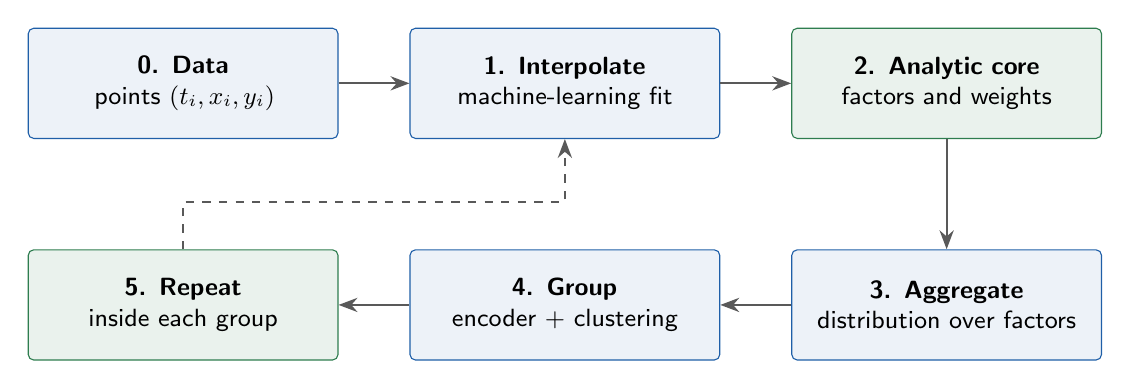
\begin{tikzpicture}[
  bx/.style={draw=cA,fill=cA!8,rounded corners=2pt,minimum height=14mm,text width=3.7cm,align=center,font=\small\sffamily},
  an/.style={draw=cC,fill=cC!10,rounded corners=2pt,minimum height=14mm,text width=3.7cm,align=center,font=\small\sffamily},
  ar/.style={-{Stealth[length=2.4mm]},thick,gray!70!black}]
\node[bx] (d) {\textbf{0. Data}\\ points $(t_i,x_i,y_i)$};
\node[bx,right=9mm of d] (i) {\textbf{1. Interpolate}\\ machine-learning fit};
\node[an,right=9mm of i] (f) {\textbf{2. Analytic core}\\ factors and weights};
\node[bx,below=14mm of f] (h) {\textbf{3. Aggregate}\\ distribution over factors};
\node[bx,left=9mm of h] (g) {\textbf{4. Group}\\ encoder $+$ clustering};
\node[an,left=9mm of g] (o) {\textbf{5. Repeat}\\ inside each group};
\draw[ar] (d)--(i); \draw[ar] (i)--(f); \draw[ar] (f)--(h); \draw[ar] (h)--(g); \draw[ar] (g)--(o);
\draw[ar,dashed] (o.north) -- ++(0,6mm) -| (i.south);
\end{tikzpicture}
\caption{The pipeline. Green boxes are the exact mathematical parts (already built); blue boxes are the machine-learning parts (to be designed). The dashed arrow is the loop: each group becomes a new data set.}
\label{fig:pipe}
\end{figure}

\begin{enumerate}[leftmargin=*]
\item \textbf{Interpolate.} A learning algorithm fits a smooth function to the data. Because data are finite, it returns not one function but \emph{many plausible ones, each with a probability}.
\item \textbf{Analytic core.} Each plausible function is handed to my algorithm. It spits out the factors that function contains and how much of the function each factor carries.
\item \textbf{Aggregate.} Add everything up, weighting by probability: we obtain a distribution (``transport appears with weight $0.7\pm0.1$, diffusion with $0.3\pm0.1$'').
\item \textbf{Group.} Use this distribution to \emph{set the parameters} of a standard grouping method (how many groups, how spread out) and cut the data into groups, so that each group ideally ``sounds like one instrument''.
\item \textbf{Repeat inside every group.} If the grouping was good, each group contains one (at most two) factors, and the tangle number is tiny. If not, regroup. When all groups are clean, the factors rebuild the equation.
\end{enumerate}

\subsection*{A tiny example, start to finish}
Suppose the (hidden) truth is
\[
u(t,x)\;=\;0.7\,e^{-(x-t)^2}\;+\;0.3\,e^{-t}\cos x .
\]
The first piece is a bump that \emph{travels} to the right with speed $1$. The second is a wave that \emph{spreads and fades}. We only see noisy samples of $u$.
\begin{itemize}[nosep]
\item \textbf{Step 1} returns many smooth curves close to $u$, each with a probability.
\item \textbf{Step 2}, applied to each curve, finds the two factors
\[
Q_1=\partial_t+\partial_x\ \ (\text{transport}),\qquad Q_2=\partial_t-\partial_x^2\ \ (\text{diffusion}),
\]
and the pieces $u_1=0.7\,e^{-(x-t)^2}$ and $u_2=0.3\,e^{-t}\cos x$.
\item \textbf{Step 3} reports: transport $\approx 70\,\%$, diffusion $\approx 30\,\%$, with their spread.
\item \textbf{Step 4} uses ``two main factors'' to choose ``two groups'' and cuts the data accordingly.
\item \textbf{Step 5} re-analyses each group alone: the first group shows only transport, the second only diffusion, and the tangle number is close to zero in both. We stop and write down the equation.
\end{itemize}

%==========================================================
\section*{Part II --- A little mathematics}
\addcontentsline{toc}{section}{Part II --- A little mathematics}

\begin{notebox}{Scope}
Everything in the analytic core assumes \textbf{exact} data and a \textbf{linear equation with constant coefficients}. This is the part I have worked out with complete proofs. The statistical wrapper (Sections~\ref{sec:wrap}--\ref{sec:loop}) is a \emph{proposal}: this is where I need you.
\end{notebox}

\subsection{Setting}
Let $u(t,x)$ be defined on a bounded region $\Omega\subset\R^2$. It satisfies a linear equation with constant coefficients $P(\partial_t,\partial_x)\,u=0$ that is \emph{not} known. Replacing $\partial_t\to\tau$, $\partial_x\to\xi$ turns an operator into a polynomial, its \emph{symbol}. Polynomials factor, and the factors are our ``instruments'':
\[
P=Q_1Q_2\cdots Q_N .
\]
For the example above, $P=(\tau+\xi)(\tau-\xi^2)$.

\subsection{The analytic core (exact data)}\label{sec:core}

\paragraph{(i) Factors generate components.}
If the $Q_j$ are pairwise coprime and $\Omega$ is simply connected, every solution splits as
\[
u=\sum_{j=1}^{N}u_j,\qquad Q_j(\partial)\,u_j=0 .
\]
The split is unique up to a finite-dimensional space of exponential-polynomials, of dimension
\[
\delta(P)=\sum_{i<j}\dim_{\mathbb C}\,\mathbb C[\tau,\xi]\big/(Q_i,Q_j).
\]
(This is the Chinese Remainder Theorem in two variables; the ambiguity is a few exponentials, not a function.) \emph{Splitting by additive terms of $P$ instead of factors is false in general.}

\paragraph{(ii) Evolution factors have an explicit projector.}
If $Q_j=\partial_t-a_j(\partial_x)$ with distinct $a_j$, then applying all the other factors kills every other component:
\[
\prod_{k\ne j}\big(\partial_t-a_k(\partial_x)\big)\,u\;=\;\prod_{k\ne j}\big(a_j-a_k\big)(\partial_x)\,u_j .
\]
So $u_j$ is recovered by ``dividing'' by $\prod_{k\ne j}(a_j-a_k)(\partial_x)$, up to its kernel (this is the finite ambiguity). In the example, $a_1=-\partial_x$, $a_2=\partial_x^2$, and the division is by $-\partial_x(1+\partial_x)$, whose kernel $\mathrm{span}\{1,e^{-x}\}$ has dimension $2=\delta(P)$.

\paragraph{(iii) Terms inside a factor.}
A single factor $\partial_t-a(\partial_x)$ may itself be a sum of \emph{terms}, $a=\sum_n a_n$ (advection, diffusion, \dots). In Fourier variables $\hat u(t,\kappa)=\int u\,e^{-i\kappa x}\dd x$,
\[
\log\hat u(t,\kappa)\;=\;\log\hat u_0(\kappa)\;+\;t\sum_{n=1}^{N} a_n(\kappa),
\]
which is \emph{linear in the terms}: they are read off by regression on monomials in $\kappa$. For advection--diffusion $u_t=-cu_x+Du_{xx}$ one finds $a_1=-ic\kappa$, $a_2=-D\kappa^2$.

\paragraph{(iv) The interaction term.}
Let $S_n(t)=e^{tA_n}$ be the evolution generated by term $n$ alone and $\Delta_n=S_n(t)-\mathrm{Id}$. Define the part of $u$ that \emph{no single term explains}:
\[
\Eint\;=\;u(t)-u_0-\sum_{n=1}^N\big(S_n(t)u_0-u_0\big).
\]
For commuting terms (constant coefficients) it has the exact closed form
\[
\Eint=\Big[\prod_{n=1}^N(\mathrm{Id}+\Delta_n)-\mathrm{Id}-\sum_{n=1}^N\Delta_n\Big]u_0,
\]
or, in Fourier variables,
\[
\widehat{\Eint}(t,\kappa)=\Big[\prod_n e^{ta_n(\kappa)}-1-\sum_n\big(e^{ta_n(\kappa)}-1\big)\Big]\hat u_0(\kappa).
\]
Its value costs $O(N)$ operations (never expand the product). Two properties give the diagnostic its meaning: $\Eint=0$ if only one term acts ($N=1$), and for $N=2$ we have $\Eint=\Delta_1\Delta_2u_0$, the \emph{product} of the two single-term effects. For advection--diffusion,
\[
\frac{|\widehat{\Eint}|}{|\hat u_0|}=\big|(e^{-ic\kappa t}-1)(e^{-D\kappa^2 t}-1)\big|\le 2 .
\]

\begin{notebox}{Two different notions of ``tangle''}
It is useful to keep two quantities apart. \textbf{Between factors}: how hard is it to separate $u_1$ from $u_2$? For two factors this is measured by the Friedrichs cosine $c_F$ (the cosine of the smallest angle between $\ker Q_1$ and $\ker Q_2$, modulo their intersection): $c_F\to1$ means the components are nearly indistinguishable. \textbf{Inside a factor}: how much do its terms interact? This is $\Eint$. A good grouping makes both small. A single factor with two real terms (advection--diffusion) is a legitimate output even though $\Eint\neq0$: there $\Eint$ is information, not an error.
\end{notebox}

\subsection{Statistical wrapper (proposal)}\label{sec:wrap}

\paragraph{Step 1: a distribution of interpolants.}
The interpolation step returns a weighted family
\[
\big\{(\hat u_s,\pi_s)\big\}_{s=1}^S,\qquad \pi_s\ge0,\quad \sum_s\pi_s=1,
\]
for instance posterior samples from a Gaussian process, a Bayesian neural network, or an ensemble. The \emph{basis functions} of this fit are the object of Question~1: they may be (a) solutions of known operators (e.g.\ $e^{\lambda t+i\kappa x}$, travelling waves), so each basis function maps directly to a factor, or (b) generic functions (networks, kernels), in which case the analytic core must extract factors from the fitted function itself.

\paragraph{Step 2: analytic core, sample by sample.}
For each $\hat u_s$ the core returns factors $Q^{(s)}_j$ (with coefficient vectors $\theta^{(s)}_j$ in the space of operator coefficients) and components $u^{(s)}_j$. Define the weight of a factor as its share of the signal,
\[
w^{(s)}_j=\frac{\|u^{(s)}_j\|}{\sum_k\|u^{(s)}_k\|},
\]
choosing the minimum-norm representative to fix the finite ambiguity. If $\hat u_s$ is a linear combination of basis functions, this is simply the (normalised) coefficient mass attached to each factor, as in the toy example, where a coefficient of $0.5$ on a basis function sends weight $0.5$ to its factor.

\paragraph{Step 3: distribution over factors.}
The result of aggregation is a weighted cloud in coefficient space,
\[
\mathcal W\;=\;\sum_{s=1}^{S}\ \pi_s\sum_{j}w^{(s)}_j\ \delta_{\theta^{(s)}_j}.
\]
From $\mathcal W$ we read: the dominant factors (modes of the cloud) with their total mass $W_j$, their means $\bar\theta_j$ and covariances $\Sigma_j$; the \emph{effective number of factors}
\[
k_{\mathrm{eff}}=\exp\Big(-\sum_j W_j\log W_j\Big);
\]
and the co-occurrence of factors across samples (which factors appear together), plus the average interaction and the average separability,
\[
\bar\rho=\sum_s\pi_s\,\frac{\|\Eint(\hat u_s)\|}{\|\hat u_s-u_0\|},\qquad \bar c_F=\sum_s\pi_s\,c_F\big(\hat u_s\big).
\]

\paragraph{Step 4: using $\mathcal W$ to set the clustering.}
My proposal (to be criticised): the number of groups is $k=\lceil k_{\mathrm{eff}}\rceil$; the initial centres are the $\bar\theta_j$; the within-group variances are the $\Sigma_j$; the encoder dimension is of the order of the number of dominant factors, and the encoder is any of PCA, SVD, an autoencoder; the grouping algorithm is any of $k$-means, a Gaussian mixture, spectral clustering.

Two natural \emph{notions of group} appear in the analytic theory, and one could use either, even different ones at different stages: (a) a group is a \emph{kernel} $\ker Q_j$, i.e.\ functions annihilated by a factor (``multiplication by the operator'' picture); (b) a group is a \emph{flow family} $\{e^{tA_n}u_0\}$, i.e.\ what a term does alone (``exponential of the operator'' picture).

\subsection{The loop}\label{sec:loop}
\begin{ideabox}[title={Algorithm (outer loop)}]
\begin{enumerate}[nosep,leftmargin=*]
\item Fit the dataset $\mathcal D$ $\Rightarrow$ $\{(\hat u_s,\pi_s)\}$.
\item Run the analytic core on every $\hat u_s$ $\Rightarrow$ $\mathcal W$ and the statistics $k_{\mathrm{eff}},\ \bar\rho,\ \bar c_F$.
\item If the groups are \emph{clean} (each has $\le2$ factors, $\bar\rho<\varepsilon_1$, $\bar c_F<\varepsilon_2$), \textbf{stop}.
\item Otherwise set the encoder and clustering parameters from $\mathcal W$, split $\mathcal D$ into $\mathcal D_1,\dots,\mathcal D_k$, and \textbf{recurse} on each $\mathcal D_g$.
\item Reconstruct the equation from the surviving factors, with their probabilities.
\end{enumerate}
\end{ideabox}

\subsection{What is known and what is not}
\begin{table}[!htb]
\centering\small
\begin{tabular}{@{}p{5.2cm}p{3.2cm}p{5.5cm}@{}}
\toprule
Statement & Status & Remark\\\midrule
Factors give components; ambiguity $\delta(P)$ & proved (exact data) & simply connected $\Omega$; fails otherwise\\
Components are in $H^m$ for all $u$ & iff sum of kernels closed & needs a gap condition ($\gamma_N>0$); not automatic\\
Closed formula for $\Eint$, cost $O(N)$ & proved & constant coefficients (commuting terms)\\
$u_0\mapsto\Eint$ continuous in $H^m$ & \textbf{false} & stability under noise is a real issue\\
Finite data certify the equation & \textbf{impossible} & no finite certificate; black box impossible\\
Nonlinear extension & partial & Burgers: closed form before the shock\\
Dictionary identification, nonlinear & exact modulo differential consequences & a countable dictionary cannot identify everything\\
Statistical wrapper (II.3--II.4) & \textbf{proposal} & no convergence or noise-robustness theory\\
\bottomrule
\end{tabular}
\caption{What the analytic theory guarantees, and what is still open.}
\end{table}

The last rows are the reason for this note: the analytic core is exact but fragile under noise, and the statistical wrapper is exactly the mechanism that could make it usable.

%==========================================================
\section*{Part III --- Questions for you}
\addcontentsline{toc}{section}{Part III --- Questions for you}

\begin{askbox}{Q1 --- Must the basis functions be chosen in advance?}
If the interpolation uses basis functions that solve known equations (exponentials for constant coefficients, travelling waves for transport, Bessel or Airy functions for others), then the method is easy to implement, but \emph{it can only discover equations whose building blocks are in the list}. For example, if there is no transport-type basis function, a transport equation may be misidentified. A fully generic fit (neural network, kernel method, Gaussian process) avoids the choice, but then the analytic core must extract factors from a function with no built-in structure.\\[3pt]
\textbf{Is there a standard way to avoid committing to a basis in advance} (e.g.\ learning the basis, a nonparametric fit followed by Fourier- or jet-based extraction, a hierarchy of dictionaries), \textbf{and what does one lose in doing so?}\\[3pt]
\emph{Relevant fact from the analytic side:} no countable dictionary identifies everything exactly, and with a fixed dictionary one only recovers an equation modulo its differential consequences. So the question is not purely technical.
\end{askbox}

\begin{askbox}{Q2 --- Designing the outer structure}
I constructed the analytic core. I would like advice on everything around it:
\begin{enumerate}[nosep,leftmargin=*]
\item \textbf{Loop and stopping rule.} Is ``recurse until each group is clean'' sensible? How to choose the thresholds $\varepsilon_1,\varepsilon_2$?
\item \textbf{Parameter estimation.} Is deriving $k$, the centres and the variances from the factor distribution $\mathcal W$ reasonable? Would you instead learn them jointly (end-to-end, EM, variational), with the analytic core as a differentiable layer?
\item \textbf{Choice of encoder and clustering.} PCA, SVD, an autoencoder; $k$-means, Gaussian mixtures, spectral methods. Which are appropriate when the ``clusters'' are defined by a differential structure rather than by distance?
\item \textbf{Uncertainty.} How should the probability from the interpolation step be propagated through a non-linear, possibly discontinuous map (the interaction term is not continuous in $H^m$)?
\item \textbf{Noise and validation.} What would a convincing experiment look like (synthetic data from known equations first)? Which baselines (SINDy, PDE-FIND, neural PDE learners) should it be compared against?
\end{enumerate}
\end{askbox}

\paragraph{Proposed way of working.}
Start with synthetic data from two or three known linear equations (transport $+$ diffusion mixtures like the example above). I supply the analytic core as a routine, together with the written proofs of the properties above; you design the outer structure and the experiments. The first deliverable would be the reconstructed factor distribution on those synthetic cases, compared against known ground truth.

\end{document}
